\documentclass{beamer}

\usepackage[utf8]{inputenc}
\usepackage[T1]{fontenc}
\usepackage{kantlipsum}
\usepackage{listings,xcolor}
\usepackage{inconsolata}
\usepackage{spverbatim}

\definecolor{dkgreen}{rgb}{0,.6,0}
\definecolor{dkblue}{rgb}{0,0,.6}
\definecolor{dkyellow}{cmyk}{0,0,.8,.3}

\lstset{
  language         = php,
  basicstyle       = \scriptsize\ttfamily,
  keywordstyle     = \color{dkblue},
  stringstyle      = \color{red},
  identifierstyle  = \color{dkgreen},
  commentstyle     = \color{gray},
  emph             =[1]{php},
  emphstyle        =[1]\color{black},
  emph             =[2]{if,and,or,else},
  emphstyle        =[2]\color{dkyellow}
  showstringspaces = false,
  numbers          = left,
  }

\usepackage{xstring}
\usepackage{catchfile}

\newcommand{\gitfolder}{.git}
\CatchFileDef{\headfull}{\gitfolder/HEAD}{}
\StrGobbleRight{\headfull}{1}[\head]
\StrBehind[2]{\head}{/}[\branch]
\CatchFileDef{\commit}{\gitfolder/refs/heads/\branch}{}
\StrGobbleRight{\commit}{1}[\longcommithash]

\newcommand{\gitrevisionlong}{%
	\longcommithash%
}

\newcommand{\gitrevisionsmall}{%
	\StrLeft{\longcommithash}{7}%
}


\title{Lazy collection}
\subtitle{Let your code procrastinate}
\institute{AFUP}
\date[2021]{Mai 2021}
\author[Pol]{Pol Dellaiera}
\logo{
    \vspace{-.3cm}
    \tikz{
        \node[opacity=0.15, inner sep=0.10cm, outer sep=0cm]{
            
\includegraphics[scale=0.35, keepaspectratio]{afup/style/logo/afup-icon+name-color}
        }
    }
}

\usetheme{afup}

% From https://jayrobwilliams.com/posts/2019/10/better-beamer
\makeatletter
\renewcommand{\itemize}[1][]{%
	\beamer@ifempty{#1}{}{\def\beamer@defaultospec{#1}}%
	\ifnum \@itemdepth >2\relax\@toodeep\else
	\advance\@itemdepth\@ne
	\beamer@computepref\@itemdepth% sets \beameritemnestingprefix
	\usebeamerfont{itemize/enumerate \beameritemnestingprefix body}%
	\usebeamercolor[fg]{itemize/enumerate \beameritemnestingprefix body}%
	\usebeamertemplate{itemize/enumerate \beameritemnestingprefix body begin}%
	\list
	{\usebeamertemplate{itemize \beameritemnestingprefix item}}
	{\def\makelabel##1{%
			{%
				\hss\llap{{%
						\usebeamerfont*{itemize \beameritemnestingprefix item}%
						\usebeamercolor[fg]{itemize \beameritemnestingprefix item}##1}}%
			}%
		}%
	}
	\fi%
	\setlength\itemsep{\fill}
	\ifnum \@itemdepth >1
	\vfill
	\fi%
	\beamer@cramped%
	\raggedright%
	\beamer@firstlineitemizeunskip%
}
\def\enditemize{\ifhmode\unskip\fi\endlist%
	\usebeamertemplate{itemize/enumerate \beameritemnestingprefix body end}
	\ifnum \@itemdepth >1
	\vfil
	\fi%
}
\makeatother

\usepackage{environ}

\newcommand{\sepframe}[2]{
    \setbeamercolor{background canvas}{bg=afupbluebackground}

    \begin{frame}[noframenumbering,plain]
        \begin{tikzpicture}[remember picture,overlay]
            \fill[afuppink] (0,0) rectangle(.05,\paperheight);
        \end{tikzpicture}
      \begin{tikzpicture}[remember picture,overlay]
          \ifx\insertframesubtitle\@empty%
              {\node[anchor=west, afupblue, font=\huge] at (0,.25){\uppercase\expandafter{#1}};}
          \else%
              {
                  \node[anchor= west, afupblue, font=\huge] at (0,.25){\uppercase\expandafter{#1}};%
                  \node[anchor= west, afuppink,font=\small] at (0,-.5){\uppercase\expandafter{#2}};}%
          \fi
      \end{tikzpicture}

      \begin{tikzpicture}[remember picture, overlay]
          \node at (current page.south east) {
              
\includegraphics[trim=0 -4cm -4cm 0, scale=.35, keepaspectratio]{src/afup/style/logo/afup-icon-color}
            };
      \end{tikzpicture}
    \end{frame}
  }

\NewEnviron{sepFrameA}[3][]{%
    \begin{frame}
        \begin{columns}
            \column{\paperwidth}
                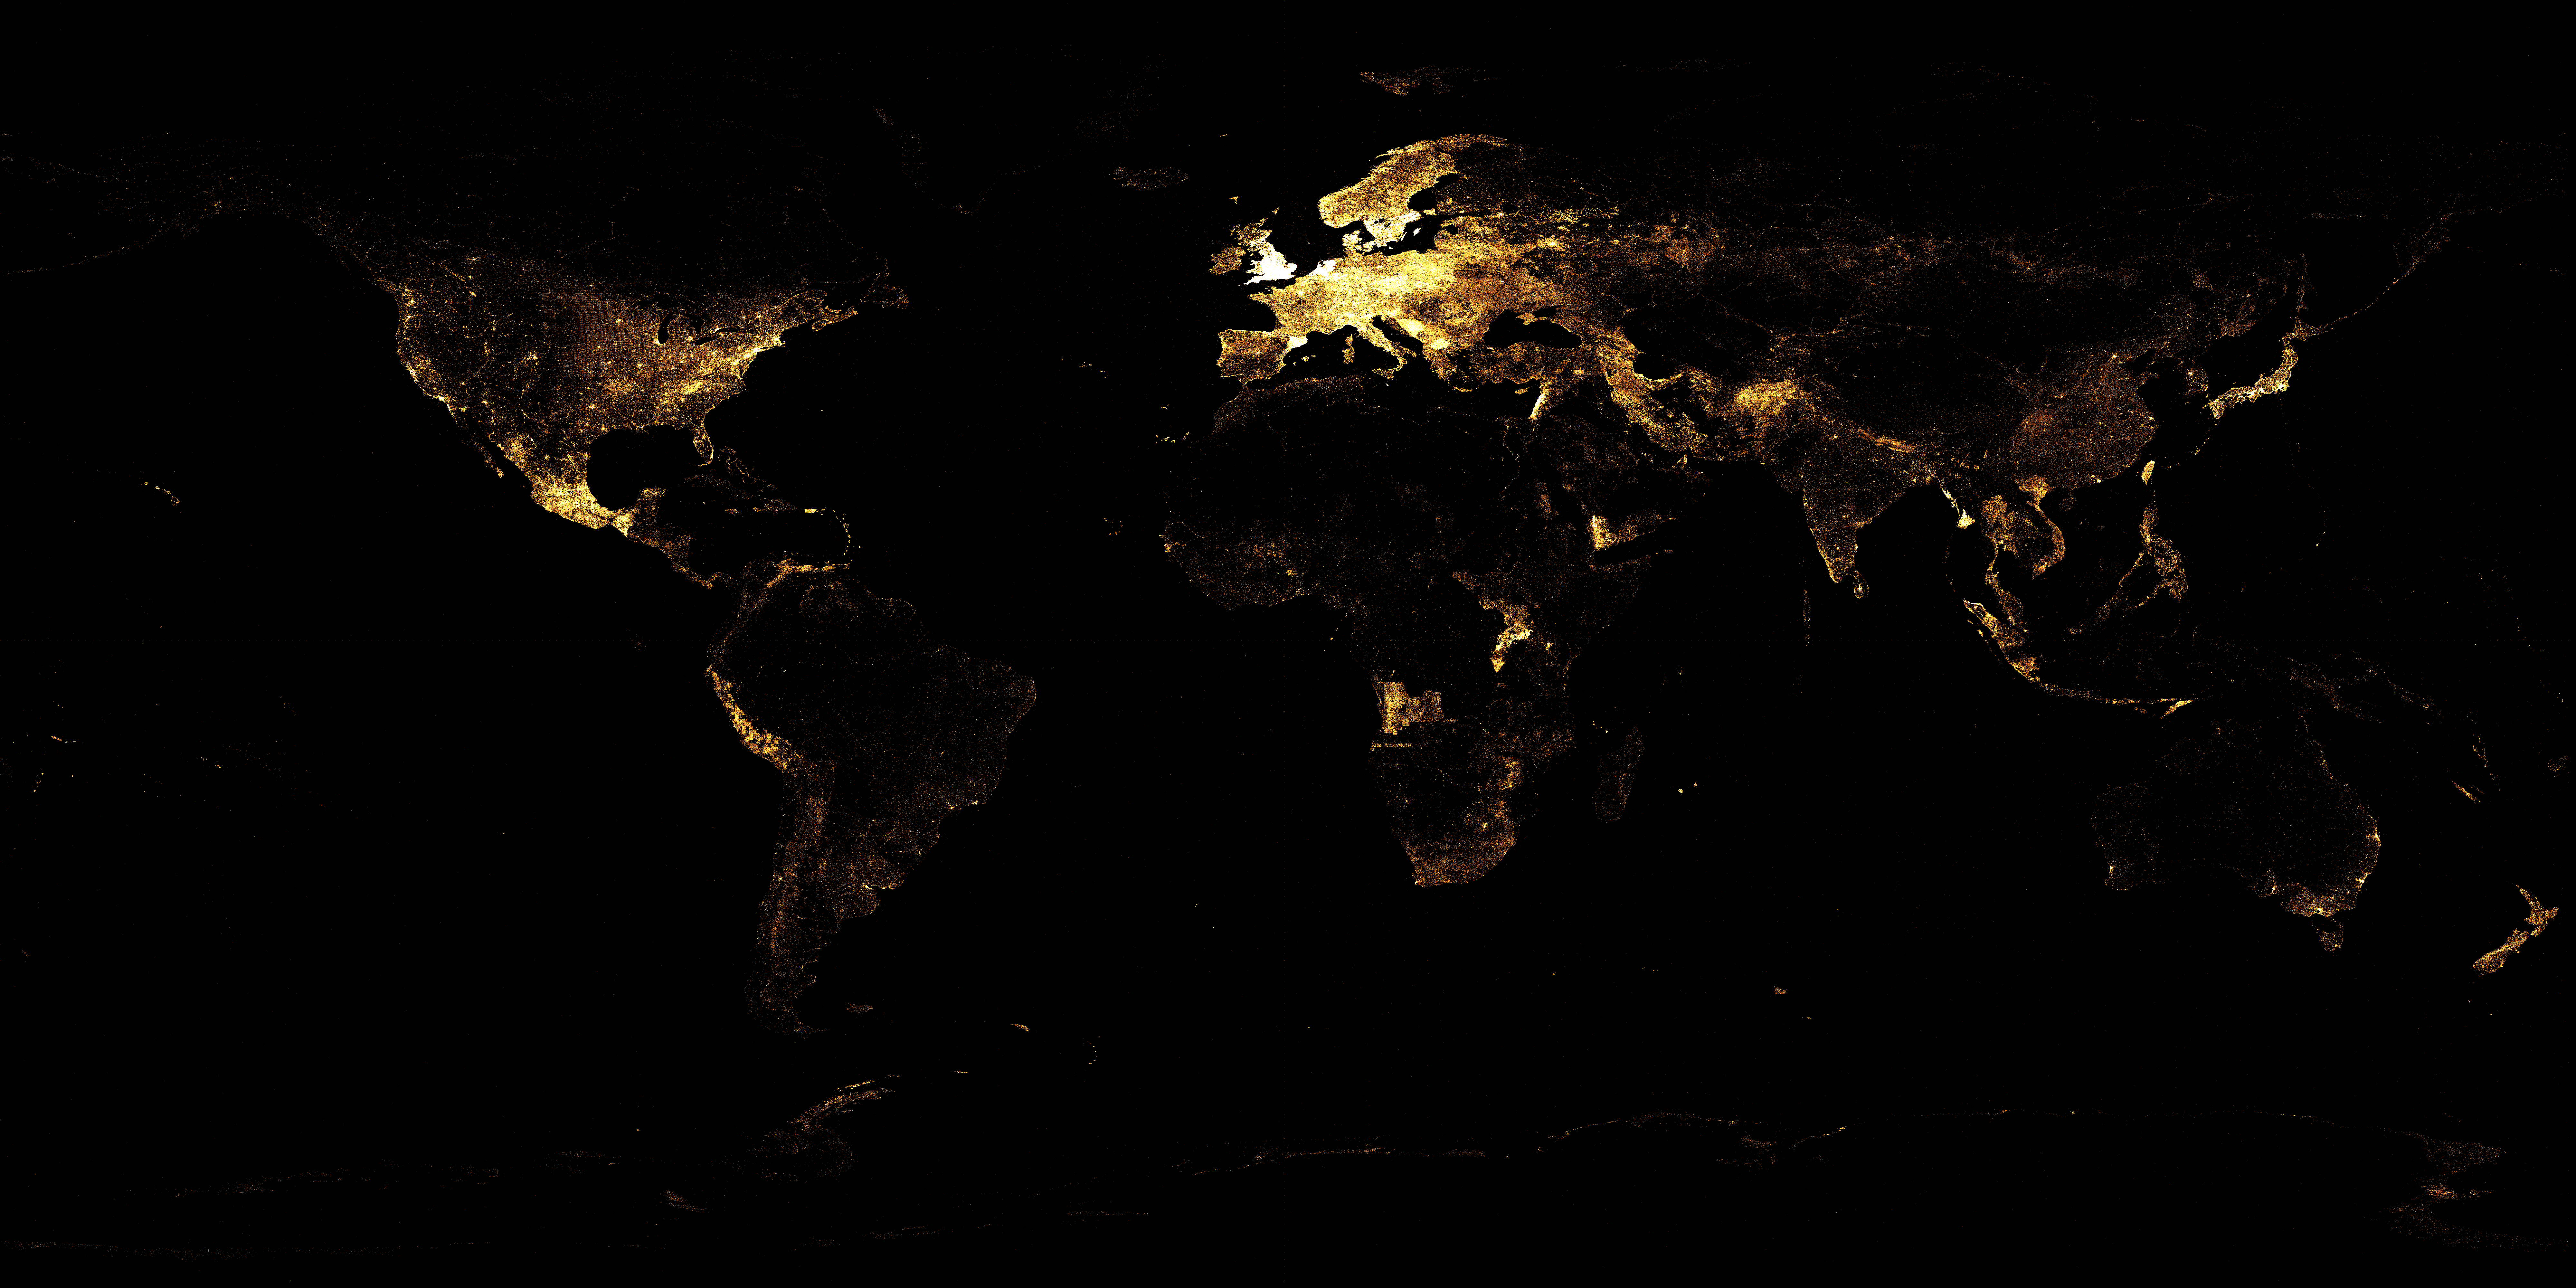
\includegraphics[width=\the\paperwidth, height=.5\paperheight]{src/afup/style/logo/bg1}
            \begin{tikzpicture}
                \node[shape=rectangle, text opacity=1,minimum height=.5\paperheight, minimum width=\paperwidth, anchor=south]{
                    \BODY
                };
            \end{tikzpicture}
          \end{columns}
    \end{frame}
}

\NewEnviron{sepFrameB}[3][]{%
    \begin{frame}
        \begin{columns}
            \column{.5\paperwidth}
                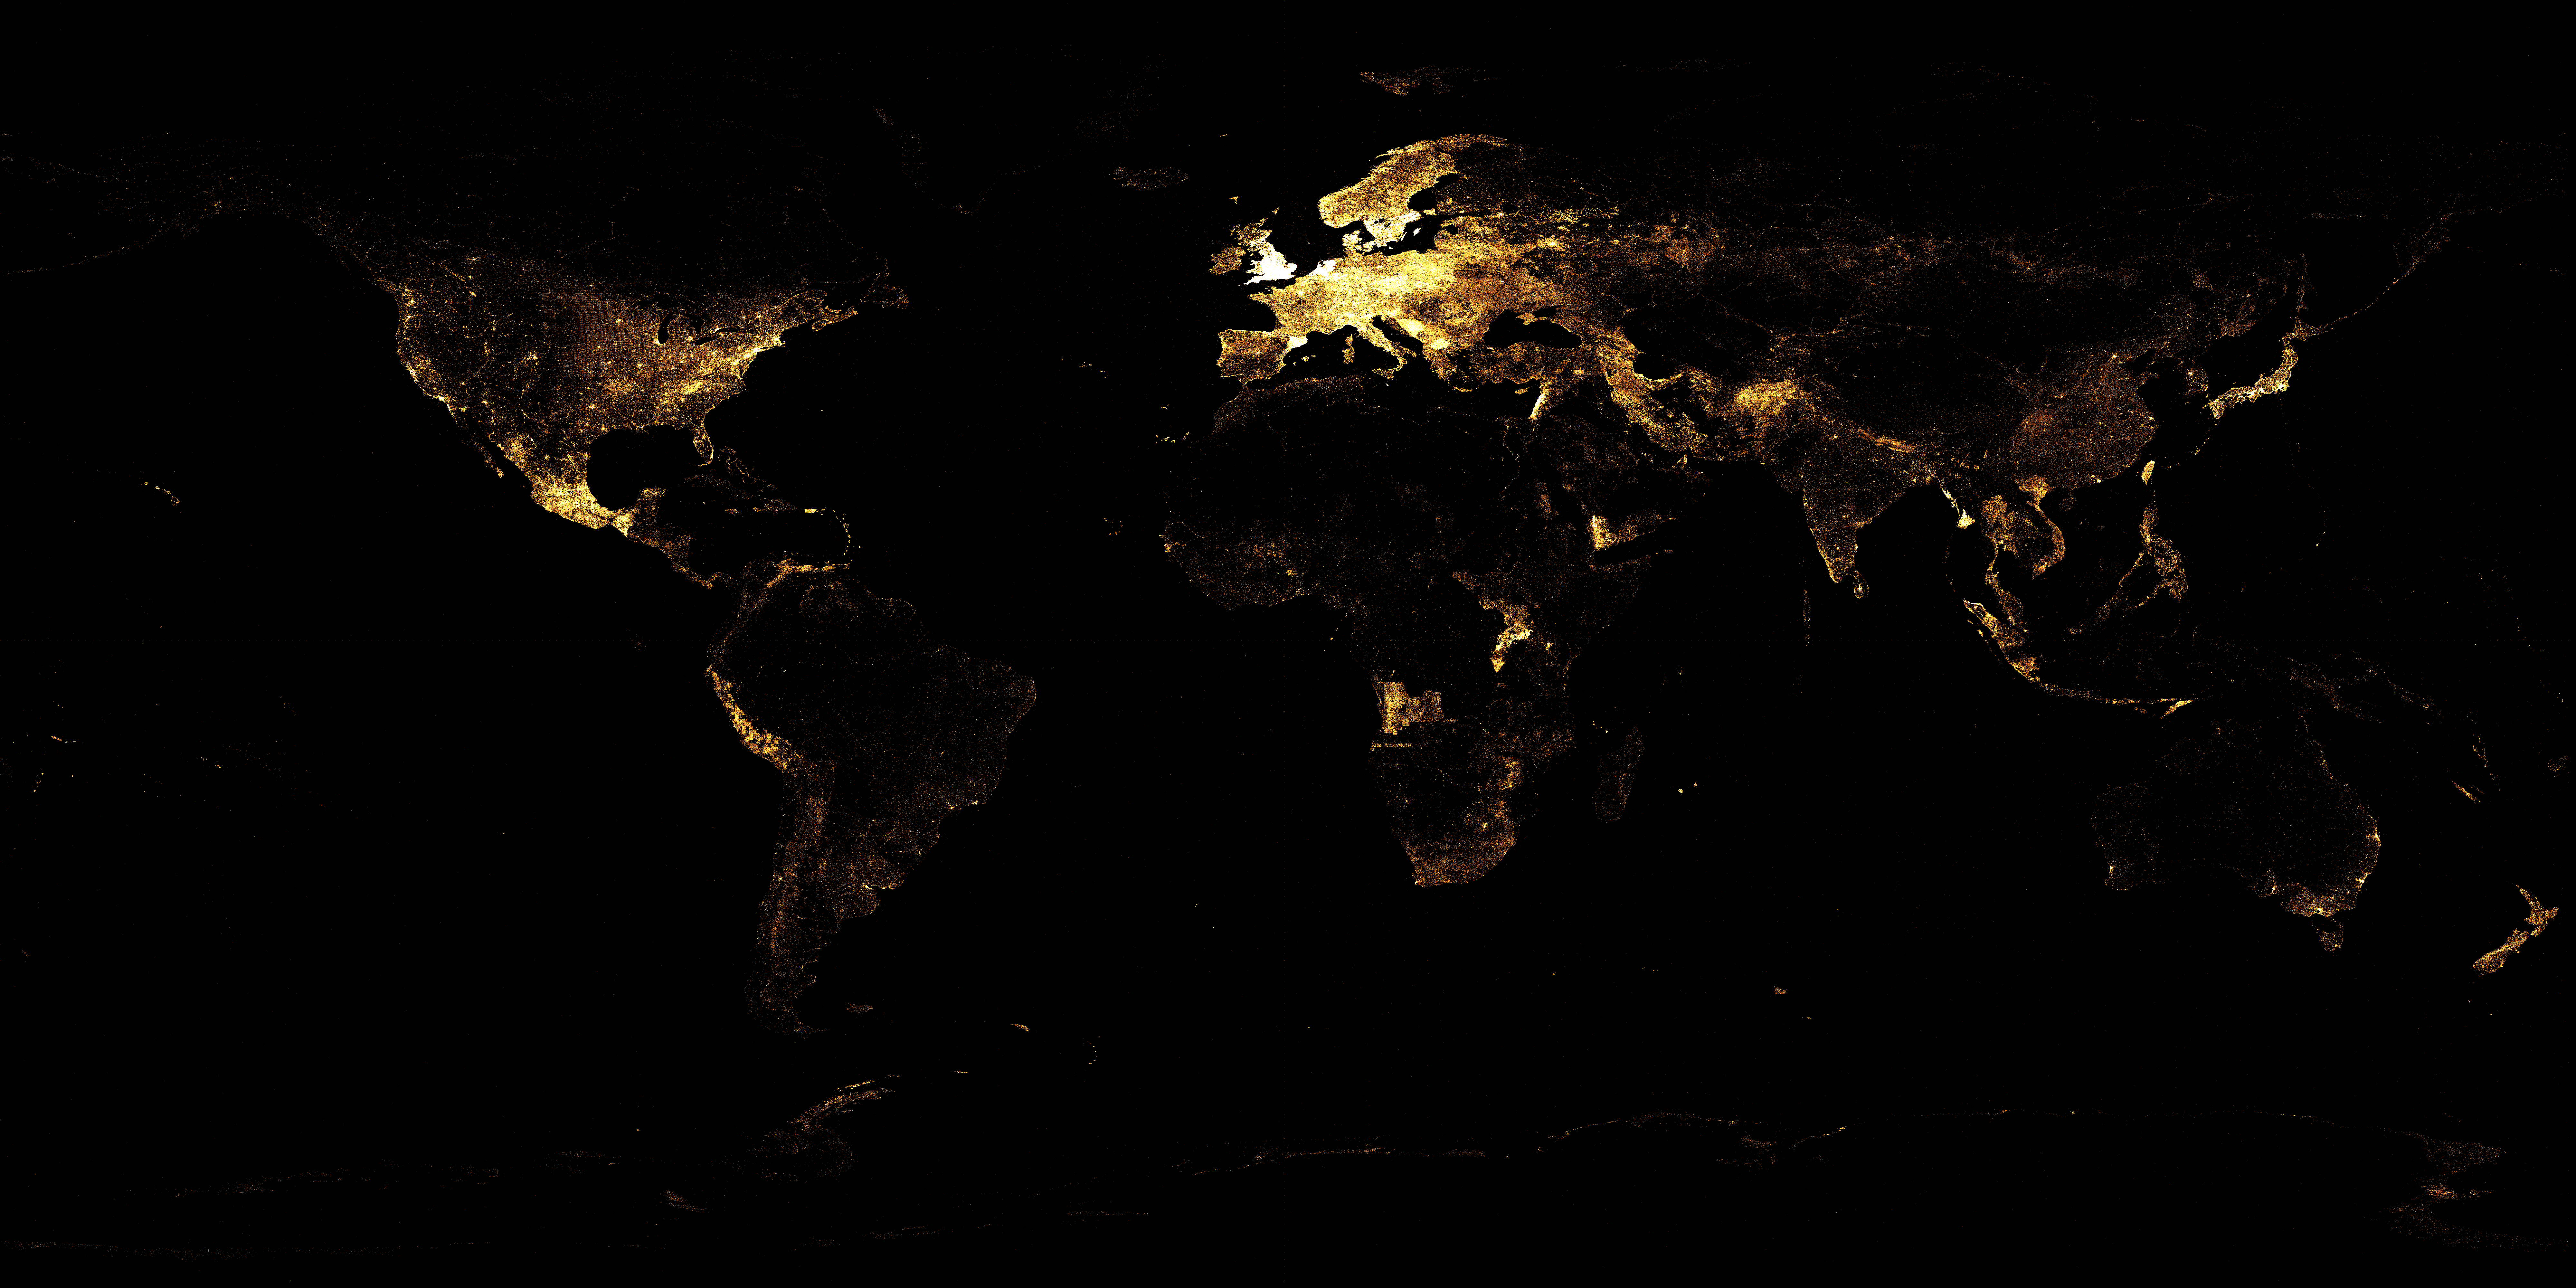
\includegraphics[width=.5\paperwidth, height=\paperheight]{src/afup/style/logo/bg1}
            \column{.5\paperwidth}
                \begin{tikzpicture}
                    \node[shape=rectangle, text opacity=1,minimum height=\paperheight, minimum width=.5\paperwidth, anchor=east]{
                        \BODY
                    };
                \end{tikzpicture}
        \end{columns}
    \end{frame}
}


% To read: https://tex.stackexchange.com/questions/113410/removing-sidebar-from-a-single-beamer-frame
% To read: https://github.com/deuslirio/UFGTeX-Presentation
% To read: https://github.com/matze/mtheme


\begin{document}

\begin{frame}[plain]
	\titlepage{}
\end{frame}

\newcommand\blankfootnote[1]{%
  \let\thefootnote\relax\footnotetext{#1}%
  \let\thefootnote\svthefootnote%
}

\begin{frame}{Le plat du jour}
    \begin{itemize}
        \item Pourquoi cette presentation
        \item Les collections
        \item Les types d'evaluation
        \item Lazy collection
    \end{itemize}
\end{frame}

\begin{frameD}{Pourquoi}{L'origine de mes recherches}

\end{frameD}

\begin{frame}
    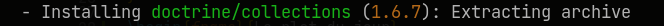
\includegraphics[width=\textwidth]{screenshots/Screenshot_20210520_104535.png}
    \pause
    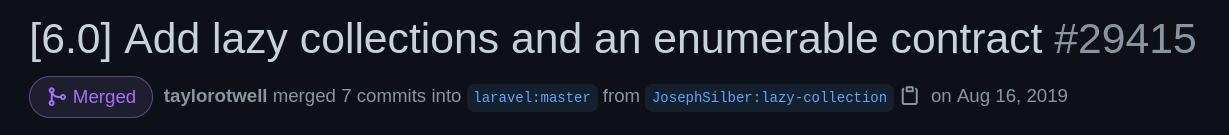
\includegraphics[width=\textwidth]{screenshots/Screenshot_20210520_101402.png}
    
\includegraphics[width=\textwidth]{screenshots/Screenshot_20210520_101458.png}
\end{frame}

\begin{frameC}{Pourtant, on a déjà tout en PHP!}

\end{frameC}

\begin{frame}{Pourquoi}{Oui mais...}
    Tout cela est déjà possible avec des simples boucles.

    En effet.

    Il y a plusieurs types de profils.
    - Les business
    - Les passionnes

    L'avantage du business c'est qu'il delivre vite
    L'avantage des passionnes c'est qu'il favoriseront plutot
    des aspects comme la sémantique et la lisibilite du code.

    Les désavantages ne sont pas nécessaires ici, je laisse aux
    participants le soin de tirer leurs conclusions.

    Du coup, comme je me situe dans le dernier profil, j'ai cree
    loophp/collection.
\end{frame}

\begin{frame}{Pourquoi}{Gérer des ensembles de données}
    PHP dispose de fonctions natives propices à l'itération

    \begin{itemize}[<+->]
        \item Les fonctions \texttt{array\_*} (\textit{$\pm$ 52 disponibles})
        \begin{itemize}[<+->]
            \item \texttt{array\_map()}
            \item \texttt{array\_filter()}
            \item \texttt{array\_reduce()}
            \item \texttt{array\_walk()}
        \end{itemize}
    \item \texttt{iterator\_to\_array()}
    \end{itemize}
\end{frame}

\begin{frame}{Pourquoi}{Gérer des ensembles de données}
    PHP dispose de structures natives propices à l'itération

    \begin{itemize}[<+->]
        \item Tableaux (\texttt{array})
        \item Objects/Interfaces (\texttt{ArrayObject}, \texttt{ArrayAccess})
        \item Itérateurs
        \item Générateurs
    \end{itemize}
\end{frame}

\begin{frame}{Pourquoi}{Gérer des ensembles de données}
    PHP dispose de structures natives propices à l'itération

    \begin{itemize}[<+->]
        \item \texttt{for}
        \item \texttt{foreach}
        \item \texttt{while}
        \item \texttt{do-while}
    \end{itemize}
\end{frame}

\begin{frameC}{Oui, mais\ldots}

\end{frameC}

\begin{frame}{Pourquoi}{Des incohérences?}
    \begin{itemize}[<+->]
        \item \texttt{array\_map()}
        \item \texttt{array\_filter()}
        \item \texttt{array\_reduce()}
        \item \texttt{array\_walk()}
    \end{itemize}
\end{frame}

\begin{frame}{Pourquoi}{Des incohérences?}
    \begin{itemize}[<+->]
        \item Uniquement pour les \texttt{array}
        \item Inconsistance des fonctions (\texttt{array\_*()})
        \item Ordre des arguments (\textit{Sera probablement different avec PHP 8})
        \begin{itemize}[<+->]
            \item \texttt{array\_map(\$callable, \$array)}
            \item \texttt{array\_map(\$array, \$callable)}
        \end{itemize}
        \item Inconsistance des callbacks
        \item Pas de vérification des types
        \item Performances
        \item Pas de gestion des erreurs
    \end{itemize}
\end{frame}

\begin{frame}{Incohérences}{\texttt{array\_map()}}
    Un array est composé de\ldots

    \begin{itemize}[<+->]
        \item clés (\texttt{\$key})
        \item valeurs (\texttt{\$value})
    \end{itemize}

    \pause[\thebeamerpauses]

    Cependant\ldots

    \pause[\thebeamerpauses]

    \begin{itemize}[<+->]
        \item Signature: \texttt{array\_map(\$callable, \$array)}
        \item Signature de \texttt{\$callable}: \texttt{\$callable(\$value)}
    \end{itemize}
\end{frame}

\begin{frame}{Incohérences}{Pourquoi?}
    \begin{itemize}[<+->]
        \item Un \texttt{array} est un ensemble de couple: $\left(\texttt{clé} \Rightarrow \texttt{valeur}\right)$
        \item \texttt{\$key} n'est pas passé au callback ?
    \end{itemize}
\end{frame}

\begin{frameC}{Bref\ldots}

\end{frameC}

\begin{frame}{Pourquoi}{In a nutshell}
    \begin{itemize}[<+->]
        \item On sait que PHP n'est pas parfait \pause[\thebeamerpauses] (\textit{mais qu'il va bientot l'etre :D})\pause[\thebeamerpauses]
        \item On a l'habitude et donc, on ne fait plus attention
        \item Cela ne nous empêche pas de construire de belles choses malgré tout
    \end{itemize}
\end{frame}


\begin{frameD}{Les collections}

\end{frameD}

\begin{frame}{Une collection}{Une définition simple}
    \begin{itemize}[<+->]
        \item \colorbox{yellow}{\textbf{Structure unifiée}} pour représenter un ensemble de données
        \item \colorbox{yellow}{\textbf{Faciliter}} les manipulations indépendamment de ce qu'elles contiennent
        \item \colorbox{yellow}{\textbf{Réduire}} l'effort tout en améliorant l'accessibilité et la lisibilité du code
        \item Favorise \colorbox{yellow}{\textbf{l'interopérabilité}} et la réutilisation
    \end{itemize}
\end{frame}

\begin{frame}{Collections}{Mais! Ca existe déjà!}
    \begin{itemize}[<+->]
        \item \texttt{doctrine/collections}
        \item \texttt{voku/Arrayy}
        \item \texttt{nikic/iter}
        \item Laravel
        \item CakePHP
    \end{itemize}
\end{frame}

\begin{frame}{Collections}{Pourquoi?}
    \begin{itemize}[<+->]
        \item \colorbox{yellow}{\textbf{Unifier}} la manière de travailler avec des ensemble de données
        \item \colorbox{yellow}{\textbf{Optimiser}} les algorithmes
        \item \colorbox{yellow}{\textbf{Faciliter}} l'emploi de certaines fonctionnalités
    \end{itemize}
\end{frame}

\begin{frame}[fragile]{Collections}{Exemple de code}
    \begin{lstlisting}[firstnumber=1]
        <?php

        $asciiRange = range(0, 255);

        $collection = Collection::fromIterable($range)
            ->filter(static fn(int $code): bool => 97 <= $code)
            ->filter(static fn(int $code): bool => 122 >= $code)
            ->map(static fn(int $code): string => chr($code))
            ->map(static fn(string $letter): string => strtoupper($letter))
            ->shuffle()
            ->limit(3);

    \end{lstlisting}
\end{frame}

\begin{frame}{Collections}{Avantages?}
    \begin{itemize}[<+->]
        \item \colorbox{yellow}{\textbf{Facile}} à lire et à comprendre
        \item \colorbox{yellow}{\textbf{Intuitif}} et simple
        \item \colorbox{yellow}{\textbf{Autocompletion}} dans l'environnement de travail (\textit{Codium, PHPStorm})
    \end{itemize}
\end{frame}

\begin{frame}{Collections}{Etats des lieux}
    \begin{itemize}[<+->]
        \item La plupart sont des wrapper de fonctions natives PHP
        \item La plupart ne fonctionnent qu'avec des \texttt{array}
        \item La plupart ne permettent pas de gérer plus de données que les
        fonctions natives
    \end{itemize}
\end{frame}

\begin{frame}{Collections}{Ce qui serait vraiment cool!}
    \begin{itemize}[<+->]
        \item Une collection devrait pouvoir gérer autant de données que l'on
        souhaite
        \item Une collection devrait nous fournir plus de fonctionnalités que
        celles que nous avons par défaut
        \item Une collection devrait gérer les différents types d'
        \texttt{iterable}.
    \end{itemize}
\end{frame}


\begin{frameD}{Types d'evaluation}{Traditionnelle et paresseuse}

\end{frameD}

\begin{frame}{Evaluation}{Les possibilites existantes}
    \begin{itemize}[<+->]
        \item Callback (thunk)
        \item Iterateur / Generateur
    \end{itemize}
\end{frame}

\begin{frame}[fragile]{Evaluation}{traditionnelle}
    \begin{lstlisting}[firstnumber=1]
        <?php

        $array = range('a', 'z');
    \end{lstlisting}
\end{frame}

\begin{frame}[fragile]{Evaluation}{traditionnelle}
    \begin{lstlisting}[firstnumber=1]
        <?php

        $array = range(0, 1000 ** 3);
    \end{lstlisting}
\end{frame}

\begin{frame}[fragile]{Evaluation traditionnelle}{Et bardaf...}
    \begin{spverbatim}
        PHP Fatal error: Allowed memory size of 536870912 bytes exhausted (tried to allocate 34359738376 bytes) in example.php on line 5
    \end{spverbatim}
\end{frame}

\begin{frame}[fragile]{Evaluation}{paresseuse via un thunk}
    \begin{lstlisting}[firstnumber=1]
        <?php

        $array = static fn (): array => range('a', 'z');
    \end{lstlisting}
\end{frame}

\begin{frame}[fragile]{Evaluation}{paresseuse via un thunk}
    \begin{lstlisting}[firstnumber=1]
        <?php

        $array = static fn (): array => range(0, 1000 ** 3);
    \end{lstlisting}
\end{frame}

\begin{frame}{Evaluation}{paresseuse}
        Un \textit{thunk} est une valeur qui est en attente d'evaluation.

        \pause

        Un \textit{thunk} est une function qui enrobe (wrap) une expression,
        pour postposer son evaluation.

        \pause

        Le terme est né comme une version humoristique du passé du verbe
        anglophone \textit{penser} (\textit{to think}).
\end{frame}

\begin{frame}[fragile]{Evaluation}{paresseuse via un generateur}
    \begin{lstlisting}[firstnumber=1]
        <?php

        function xrange($start, $end, $step = 1): Generator {
            for ($i = $start; $i <= $end; $i += $step) {
                yield $i;
            }
        }

        foreach (xrange(0, 1000 ** 3) as $value) {
            // Do stuff
        }
    \end{lstlisting}
\end{frame}

\begin{frame}{Evaluation}{Schématisons une évaluation traditionnelle}
    \newcolumntype{t}{>{\tt}c}
        \begin{center}
            \[
            \left[ \begin{array}{tt}
                0 \Rightarrow a \\
                1 \Rightarrow b \\
                2 \Rightarrow a
            \end{array} \right]
            \pause
            \xrightarrow{\texttt{array\_flip()}}
            \left[ \begin{array}{tt}
                a \Rightarrow 2 \\
                b \Rightarrow 1
            \end{array} \right]
            \pause
            \xrightarrow{\texttt{array\_flip()}}
            \left[ \begin{array}{tt}
                2 \Rightarrow a \\
                1 \Rightarrow b
            \end{array} \right]
            \]%
    \end{center}
\end{frame}

\begin{frame}{Evaluation}{Schématisons une évaluation traditionnelle}
    \newcolumntype{t}{>{\tt}c}
    \begin{center}
            \[
            \left[ \begin{array}{tt}
                0 \Rightarrow \left[ \begin{array}{tt} a \Rightarrow A\end{array} \right] \\
                1 \Rightarrow \left[ \begin{array}{tt} b \Rightarrow B\end{array} \right] \\
                2 \Rightarrow \left[ \begin{array}{tt} c \Rightarrow C\end{array} \right]
            \end{array} \right]
            \pause
            \xrightarrow{\texttt{array\_flip()}}
            \raisebox{-.5\height}{
\includegraphics[scale=0.05]{meme/No-RageFace.jpg}}
            \]%
            \texttt{Fatal error: Uncaught TypeError: Illegal offset type}
    \end{center}
\end{frame}

\begin{frame}{Schematisons}{evaluation \textit{lazy}}
    \newcolumntype{t}{>{\tt}c}
    \begin{center}
        \[
            \left[ \begin{array}{tt}
                0 \Rightarrow a \\
                1 \Rightarrow b \\
                2 \Rightarrow a
            \end{array} \right]
            \pause
            \xrightarrow{\texttt{array\_flip()}}
            \left[ \begin{array}{tt}
                \only<2->{a \Rightarrow 0} \\
                \only<4->{b \Rightarrow 1} \\
                \only<6->{a \Rightarrow 2}
            \end{array} \right]
            \pause
            \xrightarrow{\texttt{array\_flip()}}
            \left[ \begin{array}{tt}
                \only<3->{0 \Rightarrow a} \\
                \only<5->{1 \Rightarrow b} \\
                \only<7->{2 \Rightarrow a}
            \end{array} \right]
        \]
    \end{center}
\end{frame}

\begin{frame}{Schematisons}{evaluation \textit{lazy}}
    \newcolumntype{t}{>{\tt}c}
    \begin{center}
        \begin{minipage}[adjusting]{.65\textwidth}
            \begin{math}
                \left[ \begin{array}{tt}
                    0 \Rightarrow \left[ \begin{array}{tt} a \Rightarrow A\end{array} \right] \\
                    1 \Rightarrow \left[ \begin{array}{tt} b \Rightarrow B\end{array} \right] \\
                    2 \Rightarrow \left[ \begin{array}{tt} c \Rightarrow C\end{array} \right]
                \end{array} \right]
                \pause
                \xrightarrow{\texttt{array\_flip()}}\newline
                \left[ \begin{array}{tt}
                    \only<2->{\left[ \begin{array}{tt} a \Rightarrow A\end{array} \right] \Rightarrow 0} \\
                    \only<4->{\left[ \begin{array}{tt} b \Rightarrow B\end{array} \right] \Rightarrow 1} \\
                    \only<6->{\left[ \begin{array}{tt} c \Rightarrow C\end{array} \right] \Rightarrow 2}
                \end{array} \right]
                \pause
                \xrightarrow{\texttt{array\_flip()}}\newline
                \left[ \begin{array}{tt}
                    \only<3->{0 \Rightarrow \left[ \begin{array}{tt} a \Rightarrow A\end{array} \right]} \\
                    \only<5->{1 \Rightarrow \left[ \begin{array}{tt} b \Rightarrow B\end{array} \right]} \\
                    \only<7->{2 \Rightarrow \left[ \begin{array}{tt} c \Rightarrow C\end{array} \right]}
                \end{array} \right]
            \end{math}
        \end{minipage}
    \end{center}
\end{frame}



\begin{frame}
    \begin{center}
        \textit{
            Les chercheurs du Centre for Energy-Efficient Telecommunications (CEET) et des laboratoires Bell ont montré que
            les technologies de l'information et de la communication (TIC), qui englobent Internet, les vidéos, les fichiers sonores
            et autres services dans le cloud, produiraient plus de 830 millions de tonnes de CO\textsubscript{2} chaque année.\\
            Cela représente 2\% des émissions globales du principal gaz à effet de serre.\\
            Une telle quantité de CO\textsubscript{2} équivaut aux émissions de l'industrie aérienne.
        }
    \end{center}

    \blankfootnote{Source: \href{https://www.futura-sciences.com/planete/actualites/developpement-durable-emissions-co2-liees-internet-polluent-autant-avion-43802/}{Futura Sciences}}
\end{frame}

\begin{frame}
    \begin{quote}
        Je fais du vélo le matin, je voudrais ne pas respirer la poussière générée
        par ces datacenters fous fonctionnant si mal avec des algorithmes,
        car on se donne entre les mains un pouvoir qu'il ne maîtrise pas.

        \begin{flushright}
            \tiny{---Julien Pauli}
        \end{flushright}
    \end{quote}
\end{frame}

\begin{frame}
    \begin{quote}
        Si vous voulez être un meilleur programmeur, apprenez un autre language que
        le PHP. Si possible un language fonctionnel.

        \begin{flushright}
            \tiny{---Larry Garfield}
        \end{flushright}
    \end{quote}
\end{frame}

\end{document}
